\section{Signalfilterung}
In diesem Abschnitt soll die Signalfilterung genauer betrachtet werden. Dafür wird wieder der Ausgang des Generators mit dem Eingang des Analog-Digital-Wandlers verbunden. Parallel dazu wird der Ausgang des Generators mit dem Oszilloskop überwacht.

\subsection{Verschiedene Tiefpassfilterkurven}
\label{sec:VerTi}
Zuerst sollen die Filterkurven verschiedener Tiefpässe dargestellt werden. Hierzu wird am Generator ein Sinussignal ($f=100$ Hz) mit einer Rauschbandweite von 20 MHz eingestellt.\\

Für einen groben Überblick und um Unterschiede besser erkennen zu können werden alle Filterkurven in einem gemeinsamen Diagramm dargestellt (Abbildung \ref{fig:43aAll}). \\

\begin{figure}[h]
    \centering
    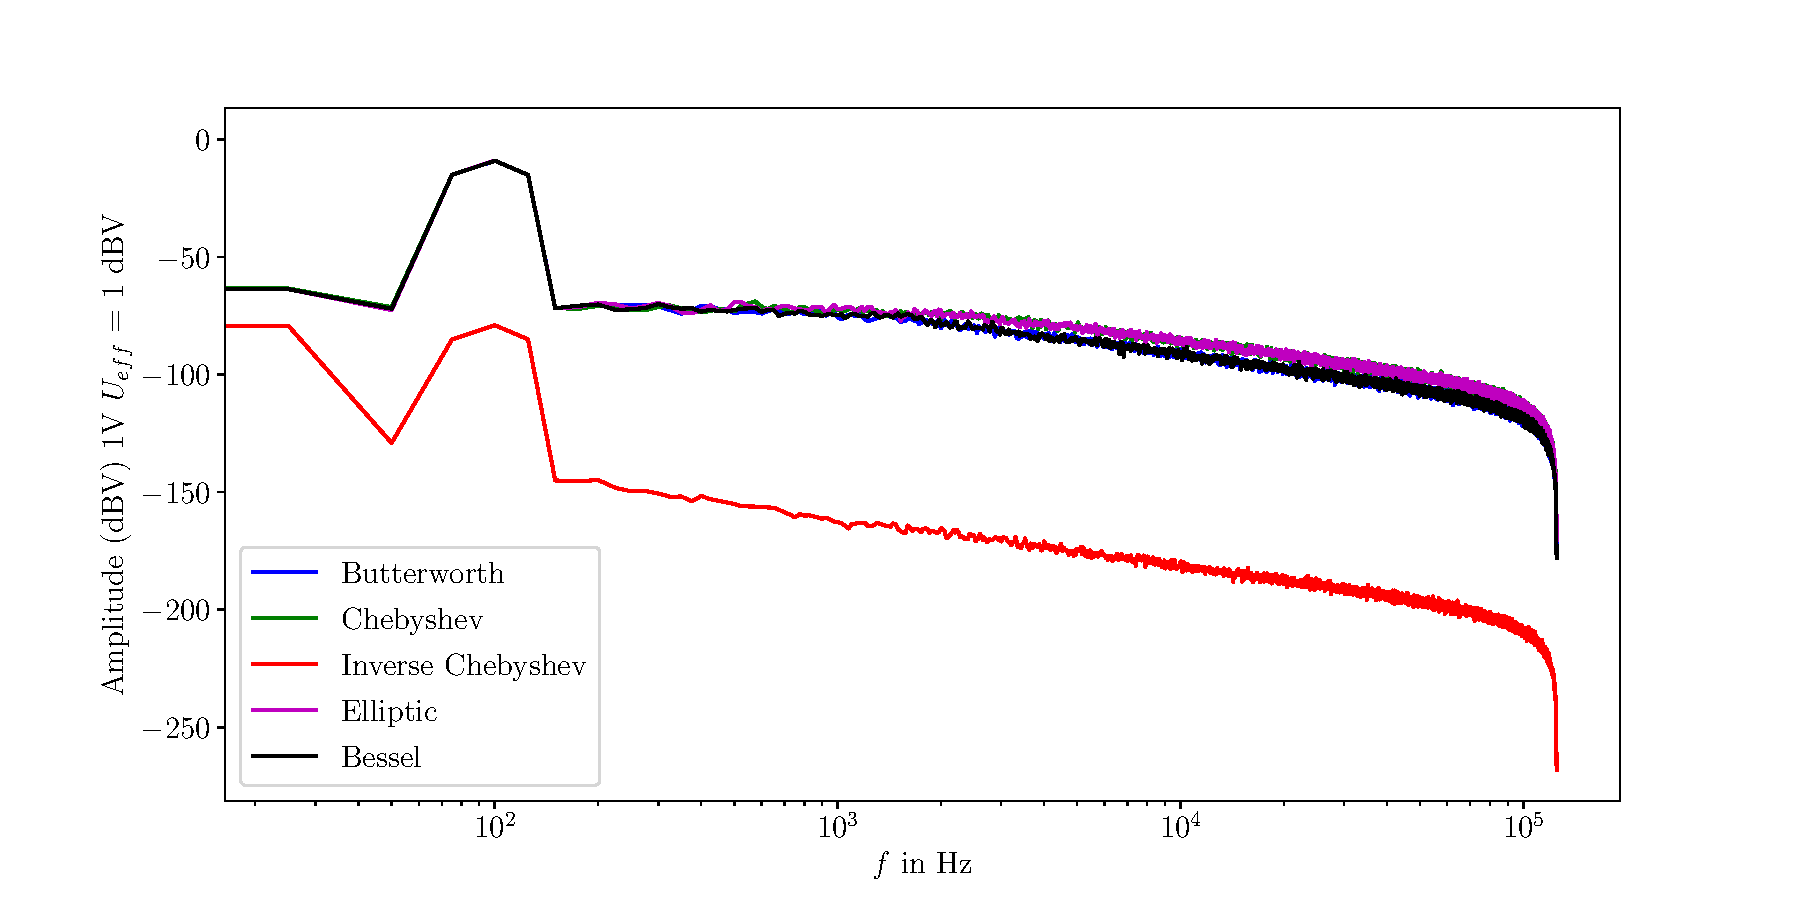
\includegraphics[width=\textwidth]{Paul/43aAll.pdf}
    \caption{Fourierspektrum verschiedene Tiefpassfilter}
    \label{fig:43aAll}
\end{figure}

In Abbildung \ref{fig:43aAll} fällt auf, dass sich Elliptic- und Chebyshevfilter fast deckungsgleich überlagern. Auch Butterworth- und Besselfilter sind auch fast deckungsgleich mit den oben genannten lediglich für Frequenzen zwischen ca. $10^3$ Hz und $10^5$ Hz divergieren sie geringfügig. Am stärksten weicht der inverse Chebyshevfilter von den anderen ab. Der Verlauf ist sehr ähnlich, nahezu parallel, jedoch ist sie Kurve nach unten verschoben. \\

\newpage
Außerdem soll  für jede Filterkurve der 3dB-Punkt und die Steigung, für große Frequenzen bestimmt werden.
Dies wurde mithilfe des Diagramms ermittelt.

\begin{table}[h]
    \centering
    \begin{tabular}[h]{l|c|c|c}
        Filter      & 3dB-Punkt in  Hz & Steigung in dB/Oktave & Steigung in dB/Dekade \\ \hline\hline
        Butterworth &    $1994\pm50$   &        $4\pm2$        &      $16\pm4$         \\ \hline
        Chebyshev   &    $1975\pm50$   &        $3\pm3$        &      $13\pm4$         \\ \hline
        inverser Chebyshev &$1499\pm50$&        $4\pm2$        &      $19\pm3$         \\ \hline
        Elliptic    &     $1499\pm50$  &        $3\pm4$        &      $15\pm6$         \\ \hline
        Bessel      &     $1801\pm50$  &        $4\pm2$        &      $17\pm4$         \\ \hline
    \end{tabular}
    \caption{Werte des 3dB-Punktes und der Steigung für verschiedene Filter}
    \label{tab:Stei}
\end{table}
Aus dem Vorbereitungsgespräch, mit dem Betreuer, ist bekannt, dass für einen Filter erster Ordnung 6 dB/Oktave (oder 20 dB/Dekade) erwartet werden. Trotz einiger Abweichungen stimmen die Größenordnungen, der Werte aus Tabelle \ref{tab:Stei} gut überein. Die großen Fehler sind der graphischen Werteermittlung geschuldet, für eine grobe Beurteilung, ob die vorliegende Messung Sinn ergib, war dies jedoch ausreichend.




\newpage
\subsection{Filterwirkung auf Rechtecksignal}
In diesem Abschnitt soll die Wirkung verschiedener Filter auf ein Rechtecksignal ($f=100$ Hz) untersucht werden.\\
Hierfür wurde der Butterworthfilter und der inverse Chebyshevfilter ausgewählt, da dieser in Abschnitt \ref{sec:VerTi} die größte Abweichung von den anderen zeigte.

\begin{figure}[h]
    \centering
    \begin{subfigure}{0.9\textwidth}
        \centering
        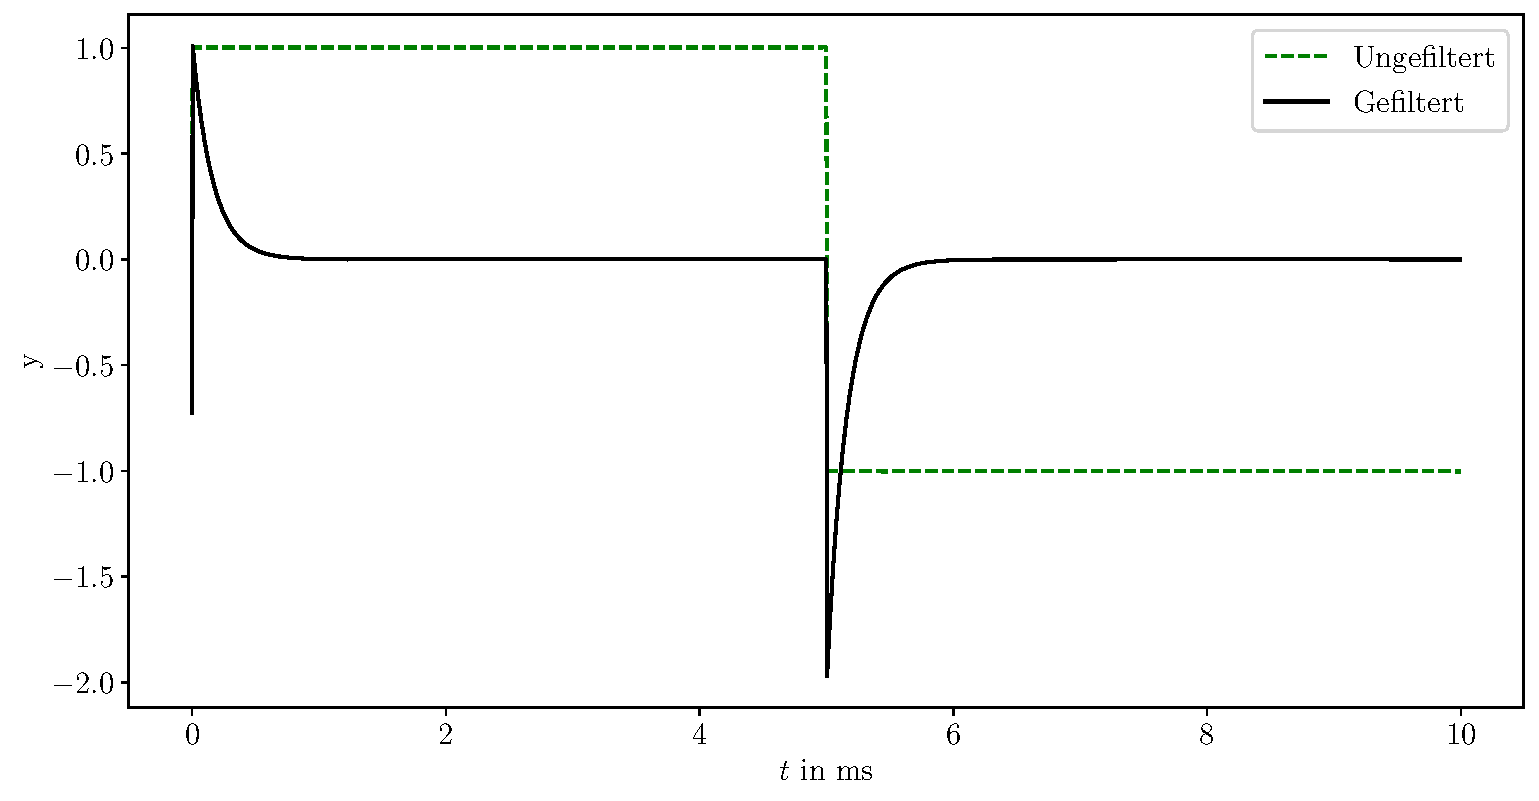
\includegraphics[width=\textwidth]{Paul/43bBuHi1S.pdf}
        \caption{Signal}
    \end{subfigure}
    \\
    \begin{subfigure}{0.9\textwidth}
        \centering
        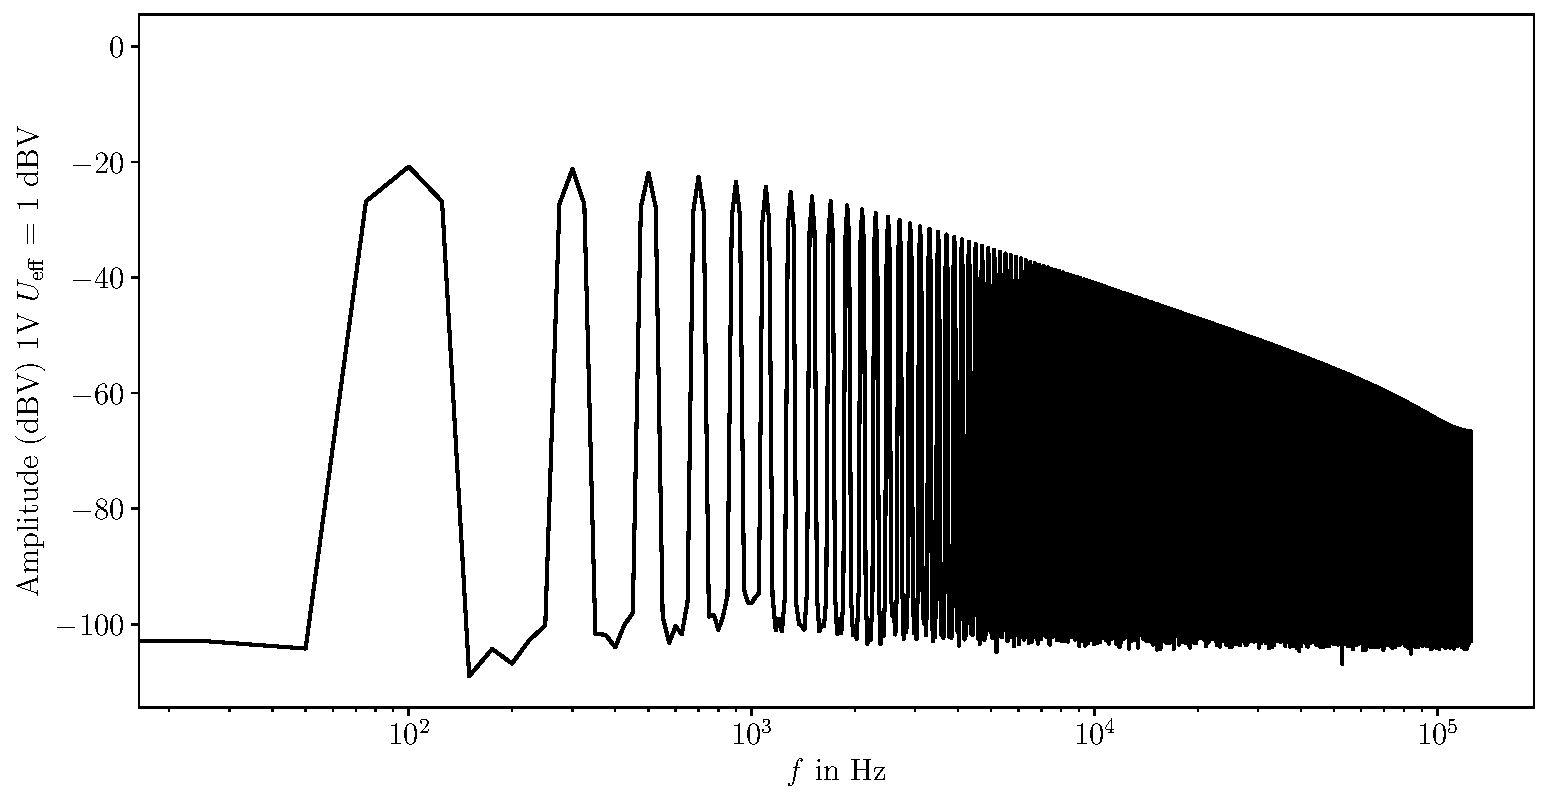
\includegraphics[width=\textwidth]{Paul/43bBuHi1F.pdf}
        \caption{Fourierspektrum}
    \end{subfigure}
    \caption{Butterworthfilter als Hochpass}
    \label{fig:43bBuHi1}
\end{figure}

Aus Abbildung \ref{fig:43bBuHi1} geht klar die differenzierende Eigenschaft des Hochpasses hervor. Außerdem knickt das Fourierspektrum für große Frequenzen nicht ab.\\

\begin{figure}[h]
    \centering
    \begin{subfigure}{0.9\textwidth}
        \centering
        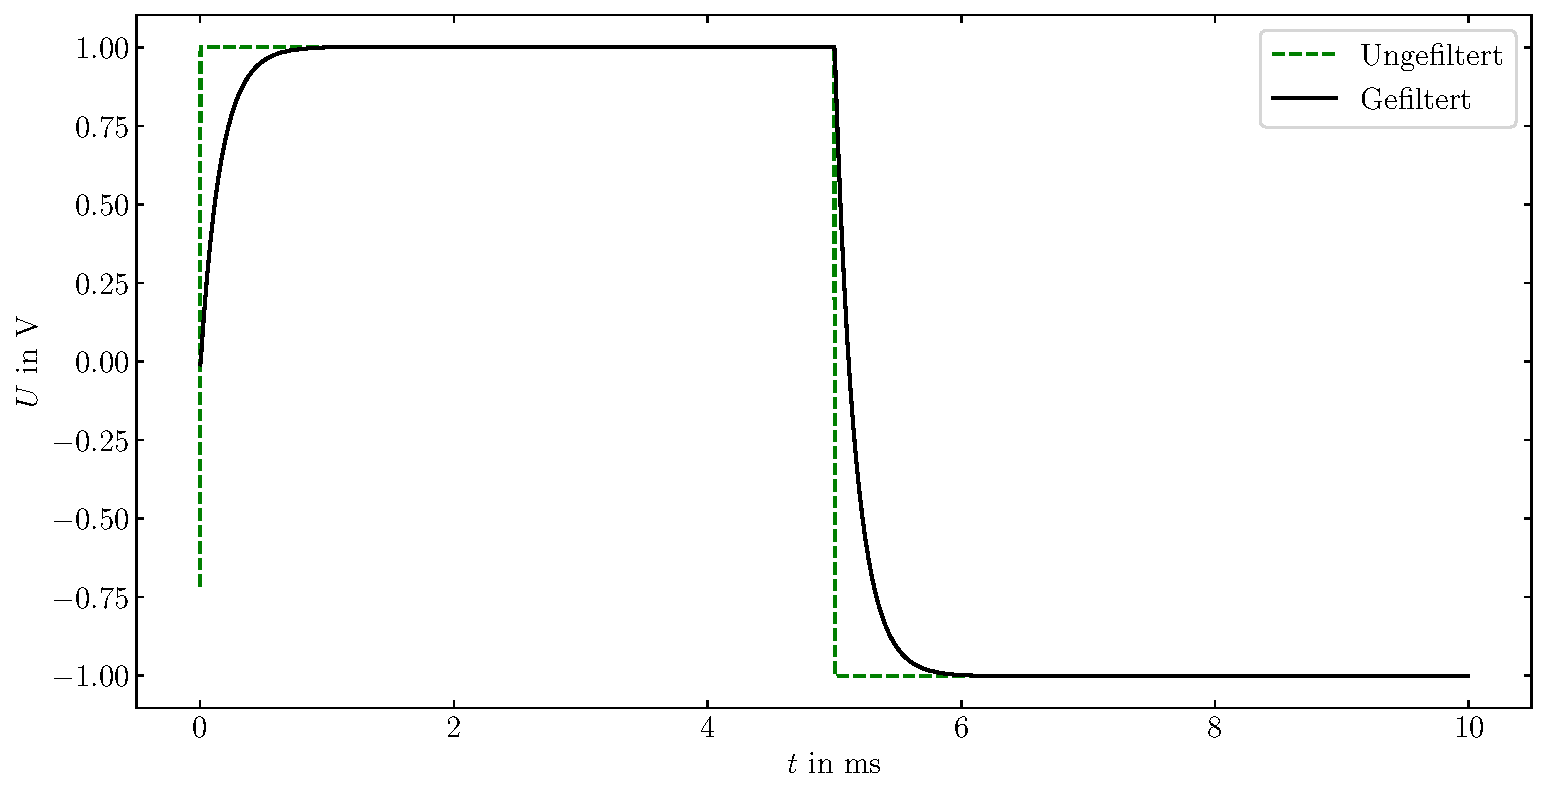
\includegraphics[width=\textwidth]{Paul/43bBuLo1S.pdf}
        \caption{Signal}
    \end{subfigure}
    \\
    \begin{subfigure}{0.9\textwidth}
        \centering
        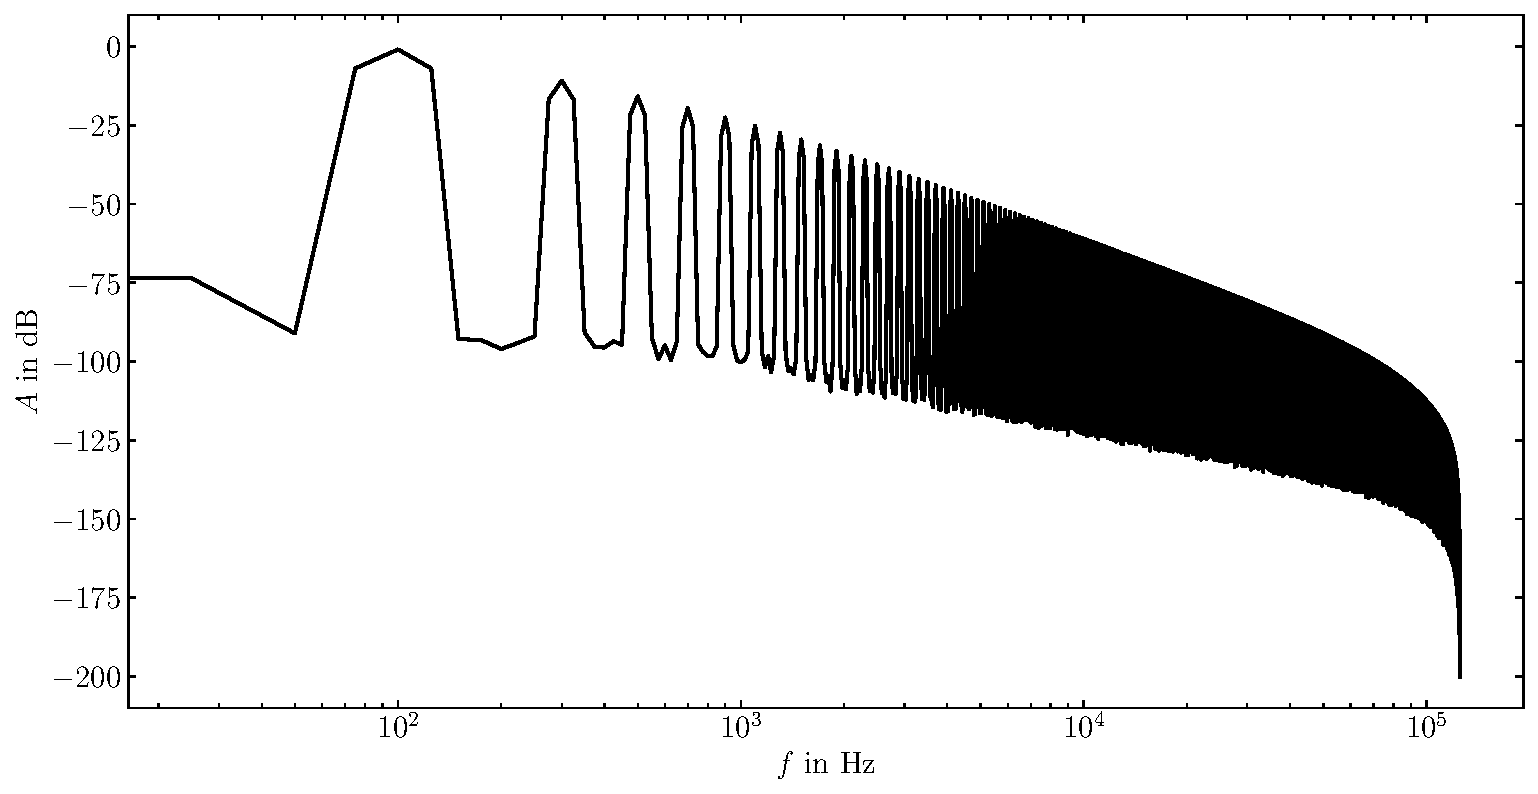
\includegraphics[width=\textwidth]{Paul/43bBuLo1F.pdf}
        \caption{Fourierspektrum}
    \end{subfigure}
    \caption{Butterworthfilter als Tiefpass}
    \label{fig:43BuLo1}
\end{figure}

Im Gegensatz zum Hochpass wirkt der Butterworthfilter Tiefpass als Integriere und das Fourierspektrum knickt für große Frequenzen ab, dies ist in Abbildung \ref{fig:43BuLo1} zu erkennen.


\newpage
Der inverse Chebyshevfilter zeigt vor allem im Signal ein ganz anderes Bild.\\
In Abbildung \ref{fig:43bInChHi1} ist beim Signal in der ersten Millisekunde eine gewisse Welligkeit zu erkennen. Im Bezug auf das Fourierspektrum fällt auf das dieser Filter, im Vergleich zum Butterworthhochpass, für größere Frequenzen schneller durchlässiger wird.
\begin{figure}[h]
    \centering
    \begin{subfigure}{0.9\textwidth}
        \centering
        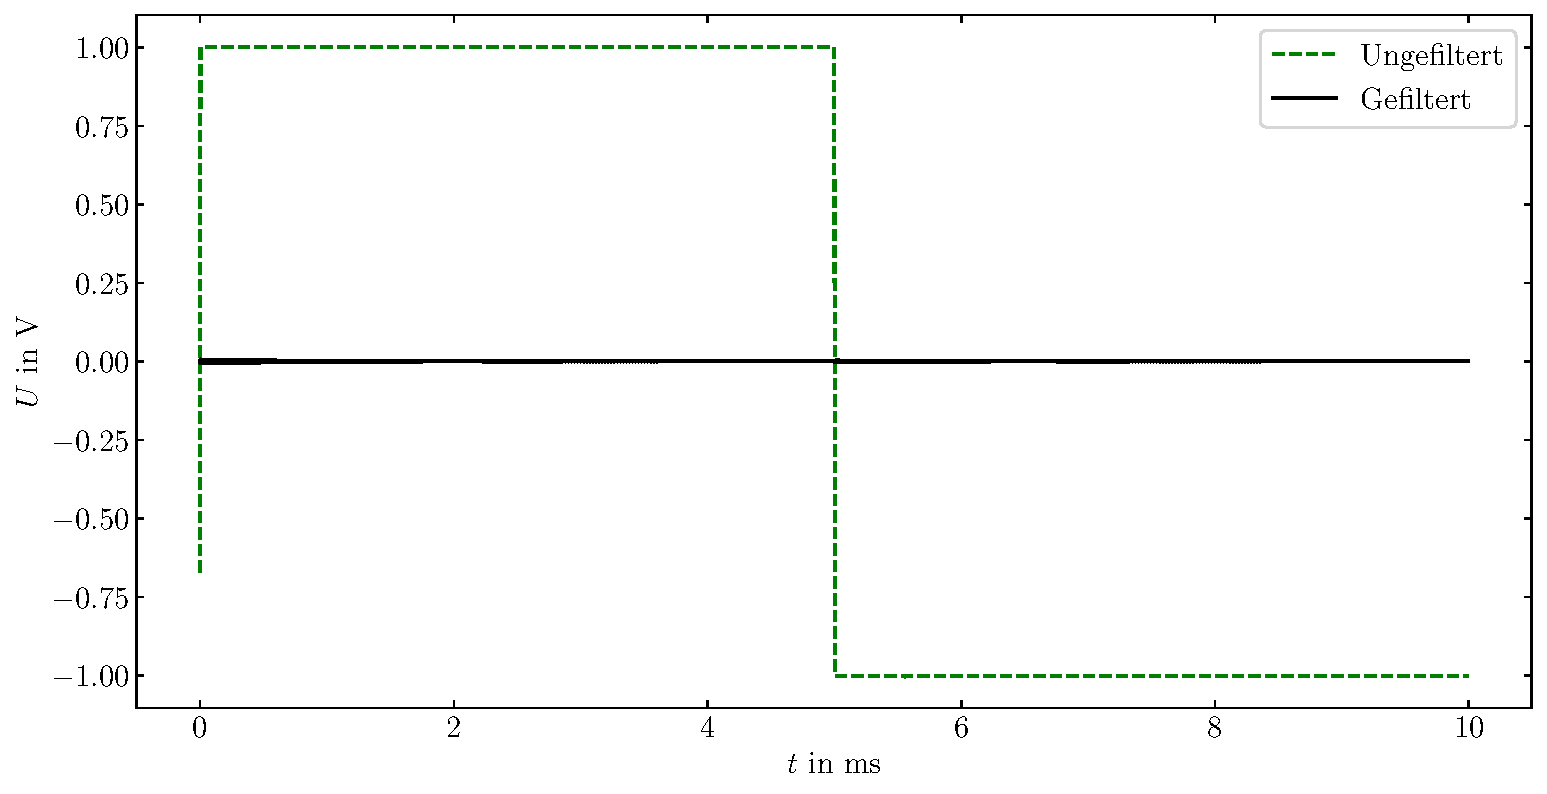
\includegraphics[width=\textwidth]{Paul/43bInChHi1S.pdf}
        \caption{Signal}
    \end{subfigure}
    \\
    \begin{subfigure}{0.9\textwidth}
        \centering
        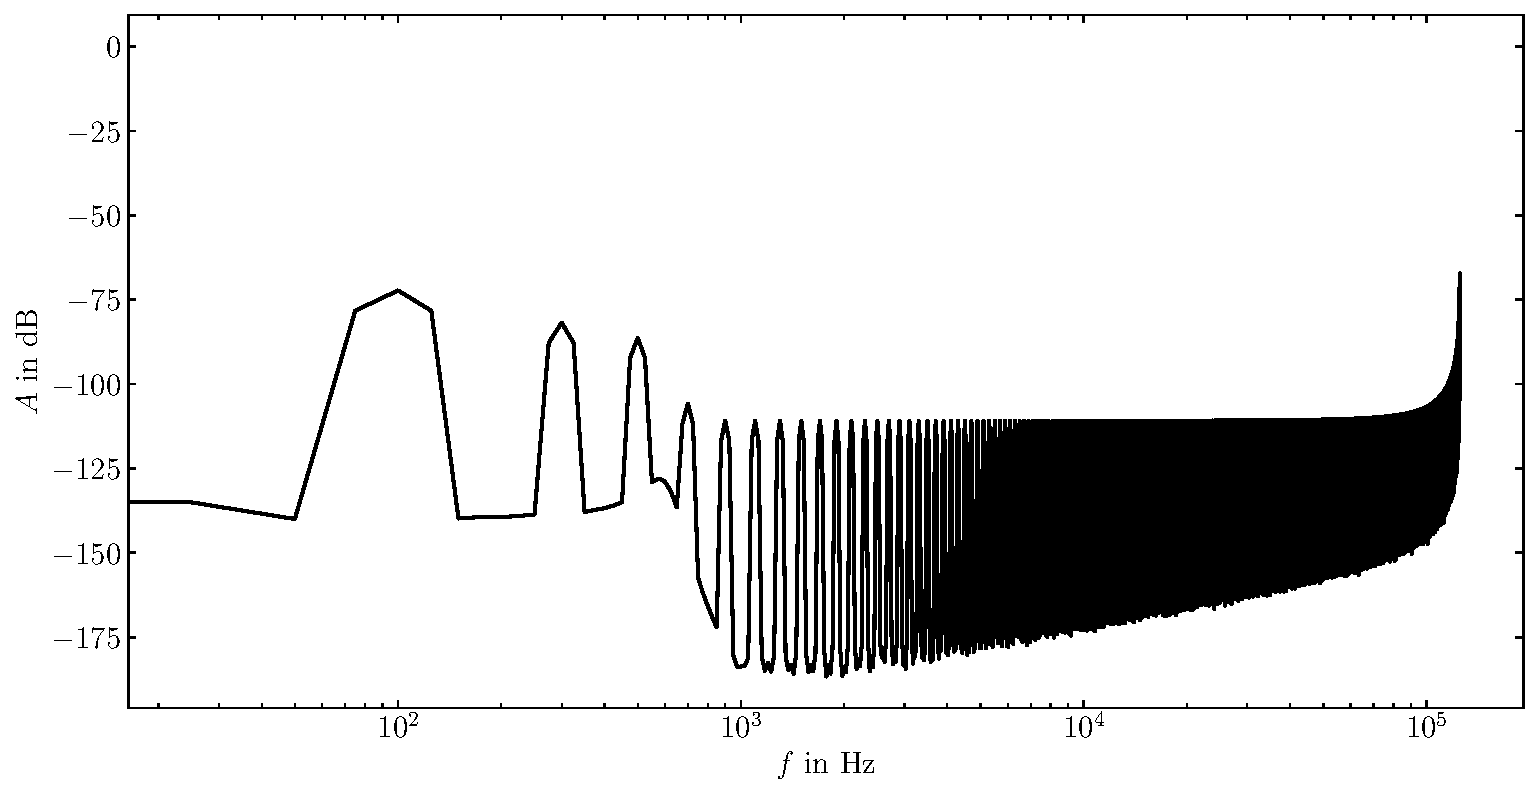
\includegraphics[width=\textwidth]{Paul/43bInChHi1F.pdf}
        \caption{Fourierspektrum}
    \end{subfigure}
    \caption{Inverser Chebyshevfilter als Hochpass}
    \label{fig:43bInChHi1}
\end{figure}

\newpage
In Abbildung \ref{fig:43bInChLo1} fällt die konstante Nulllinie beim gefilterten Signal auf, auch ist das abknicken, im Vergleich zum Butterworthtiefpass ausgeprägter.\\

\begin{figure}[h]
    \centering
    \begin{subfigure}{0.9\textwidth}
        \centering
        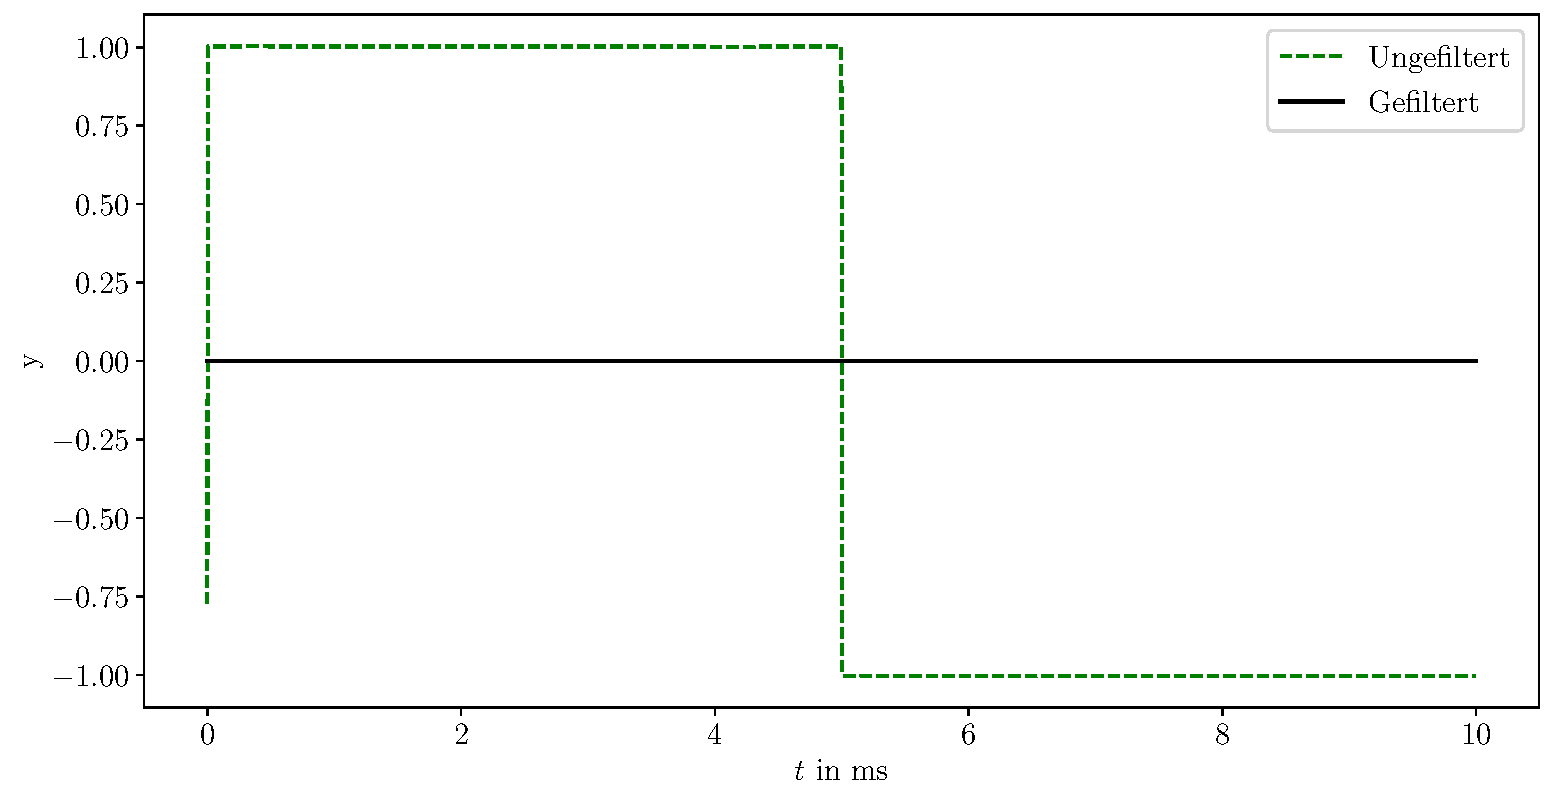
\includegraphics[width=\textwidth]{Paul/43bInChLo1S.pdf}
        \caption{Signal}
    \end{subfigure}
    \\
    \begin{subfigure}{0.9\textwidth}
        \centering
        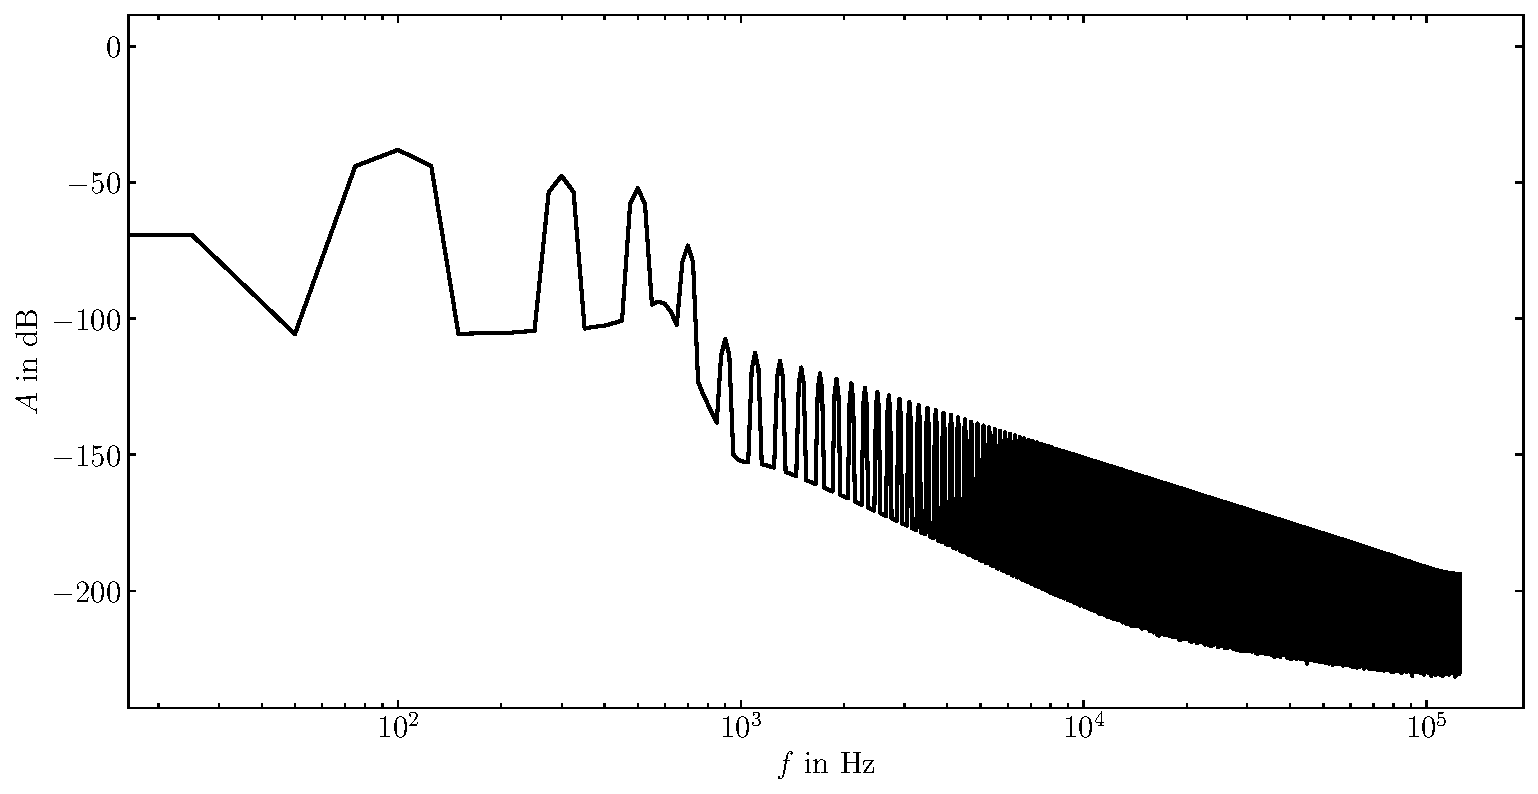
\includegraphics[width=\textwidth]{Paul/43bInChLo1F.pdf}
        \caption{Fourierspektrum}
    \end{subfigure}
    \caption{Inverser Chebyshevfilter als Tiefpass}
    \label{fig:43bInChLo1}
\end{figure}

Da die anderen Filter ähnliche Eigenschaften wie der Butterworthfilter aufweisen wurde auf die Abbildung deren Signale und Fourierspektren bewusst verzichtet.\\

\newpage
\subsection{Bandpass 4. Ordnung}

In diesem Abschnitt soll die geeignete Einstellung eines Bandpasses (4. Ordnung) gefunden werden, der Rauschen, beim gleichzeitigen Erhalt der zeitlichen Form der Signalfunktion, abgemildert werden.
\begin{figure}[h]
    \centering
    \begin{subfigure}{0.9\textwidth}
        \centering
        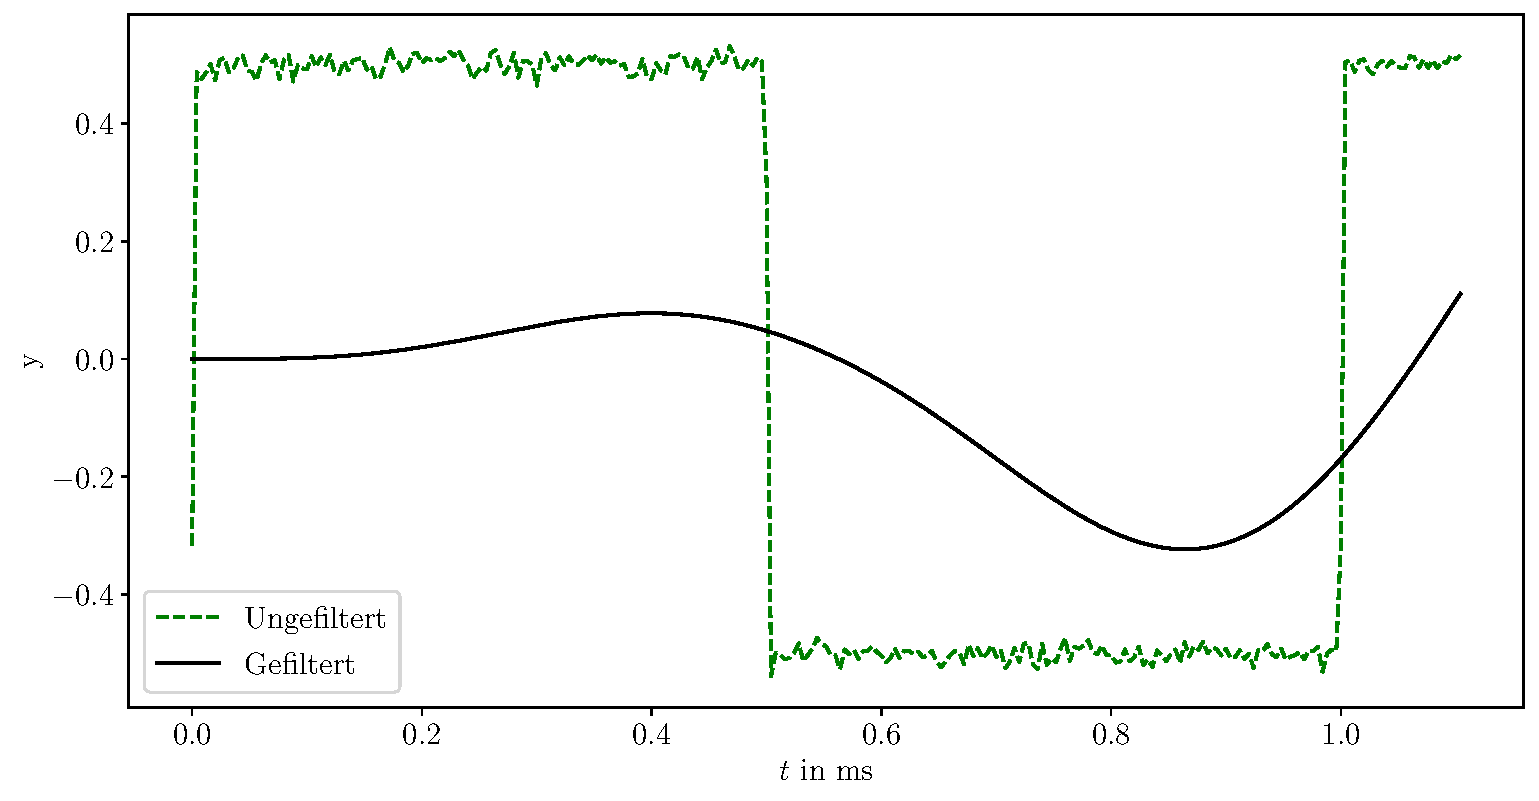
\includegraphics[width=\textwidth]{Paul/43cLf500Hf1500S.pdf}
        \caption{Bandpass mit Durchlassbereich von 500 bis 1500 Hz}
    \end{subfigure}
    \\
    \begin{subfigure}{0.9\textwidth}
        \centering
        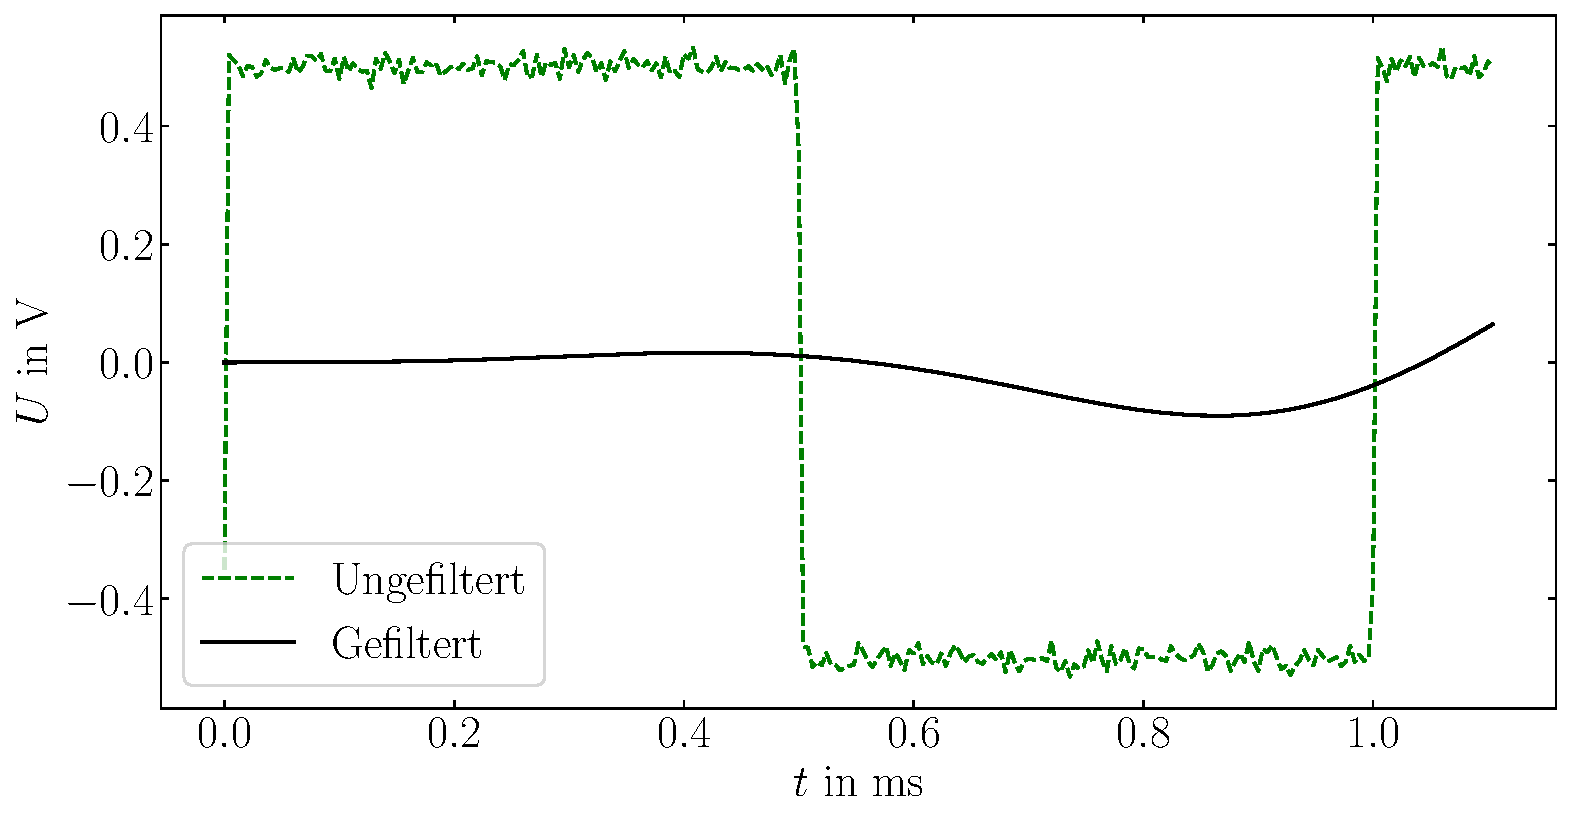
\includegraphics[width=\textwidth]{Paul/43cLf700Hf1300S.pdf}
        \caption{Bandpass mit Durchlassbereich von 700 bis 1300 Hz}
    \end{subfigure}
    \caption{Signalfunktion verschiedener Bandpässe}
    \label{fig:43cverBa}
\end{figure}

Die in Abbildung \ref{fig:43cverBa} gezeigten Signalfunktionen weichen stark von einer Rechteckfunktion ab und sind daher ungeeignet.\\
Durch weiteres ausprobieren wurden bessere Einstellungen gefunden, welche die in Abbildung \ref{fig:43cBeBa} dargestellte Signalfunktion ergeben. Hier ist noch deutlich ein Rechtecksignal zu erkennen.\\

\begin{figure}[h]
    \centering
    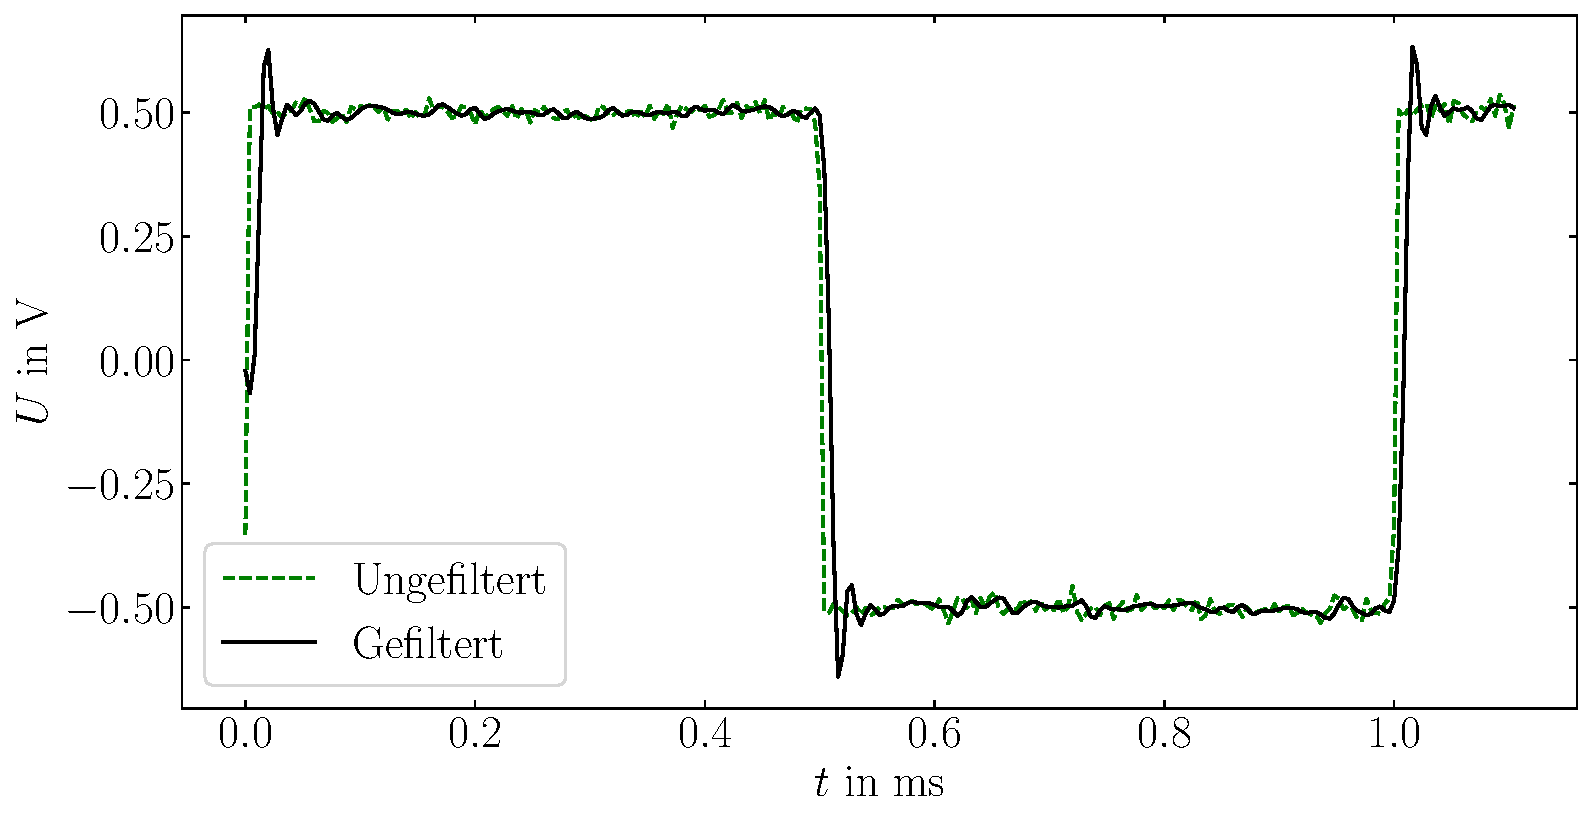
\includegraphics[width=\textwidth]{Paul/43cLf10mHz55kHzS.pdf}
    \caption{Bandpass mit Durchlassbereich von 10 mHz bis 55 kHz}
    \label{fig:43cBeBa}
\end{figure}

Eine gute Rauschunterdrückung verursacht also eine große Signalverzerrung. Es ist also darauf zu achten, dass dieses Verhältnis, abhängig vom Fokus der Messung, klug gewählt wird.

\newpage
\subsection{Einfluss der Ordnung}
Nun Stellen wir uns die Frage, welchen Einfluss die Ordnung eines Filters auf das Ausgangssignal hat.\\
Zuerst soll der Begriff Ordnung erklärt werden. Die Ordnung besagt, wie oft der gleiche Filter hintereinander geschaltet wird. Bei einem Filter der Ordnung zwei durchläuft das Signal also zweimal hintereinander einen baugleichen Filter.\\

Um den Einfluss der Ordnung genauer betrachten zu können werden Fourierspektren von Filtern verschiedener Ordnung miteinander verglichen.

\begin{figure}[h]
    \centering
    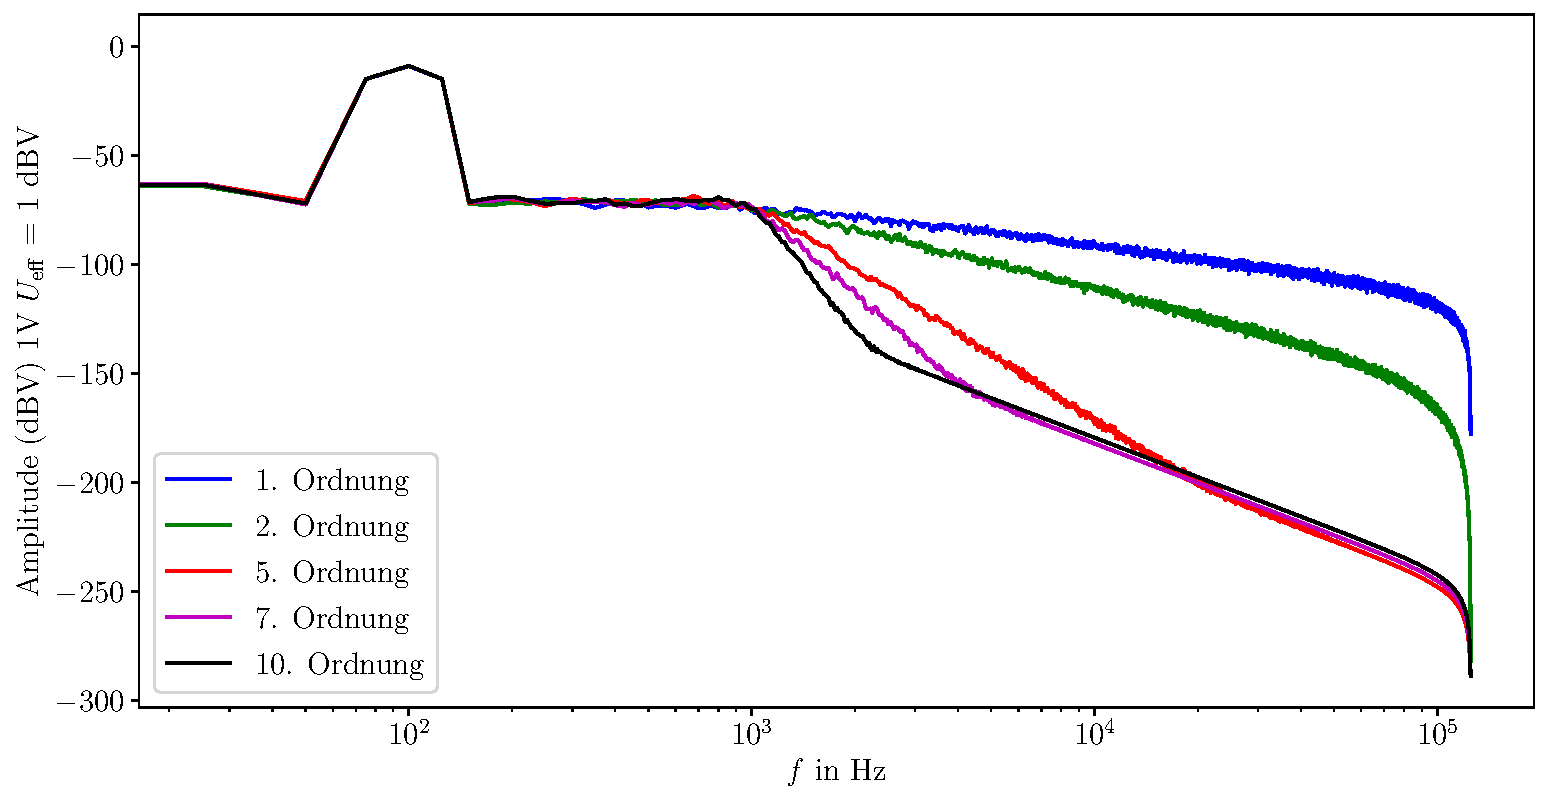
\includegraphics[width=\textwidth]{Paul/43dOrdnungF.pdf}
    \caption{Butterworthfilter bei verschiedenen Ordnungen}
    \label{fig:43dOrd}
\end{figure}

Aus Abbildung \ref{fig:43dOrd} ist zu erkennen, dass mit höherer Ordnung die Funktion steiler Abfällt.

\newpage
\subsection{Vergleich: Analoge und digitale Filterung}
Um die analoge mit der digitalen Filterung zu Vergleichen wird zuerst eine Messung mit dem gewohntem Messaufbau für den digitalen Filter aufgenommen. Danach wird der digitale Filter über die Messsoftware deaktiviert und zwischen den Generator und Detektor wird ein analoger Filter (Modell: Ithaco 4302) geschaltet, der analog zum digitalen Filter eingestellt wurde.

\begin{figure}[h]
    \centering
    \begin{subfigure}{0.9\textwidth}
        \centering
        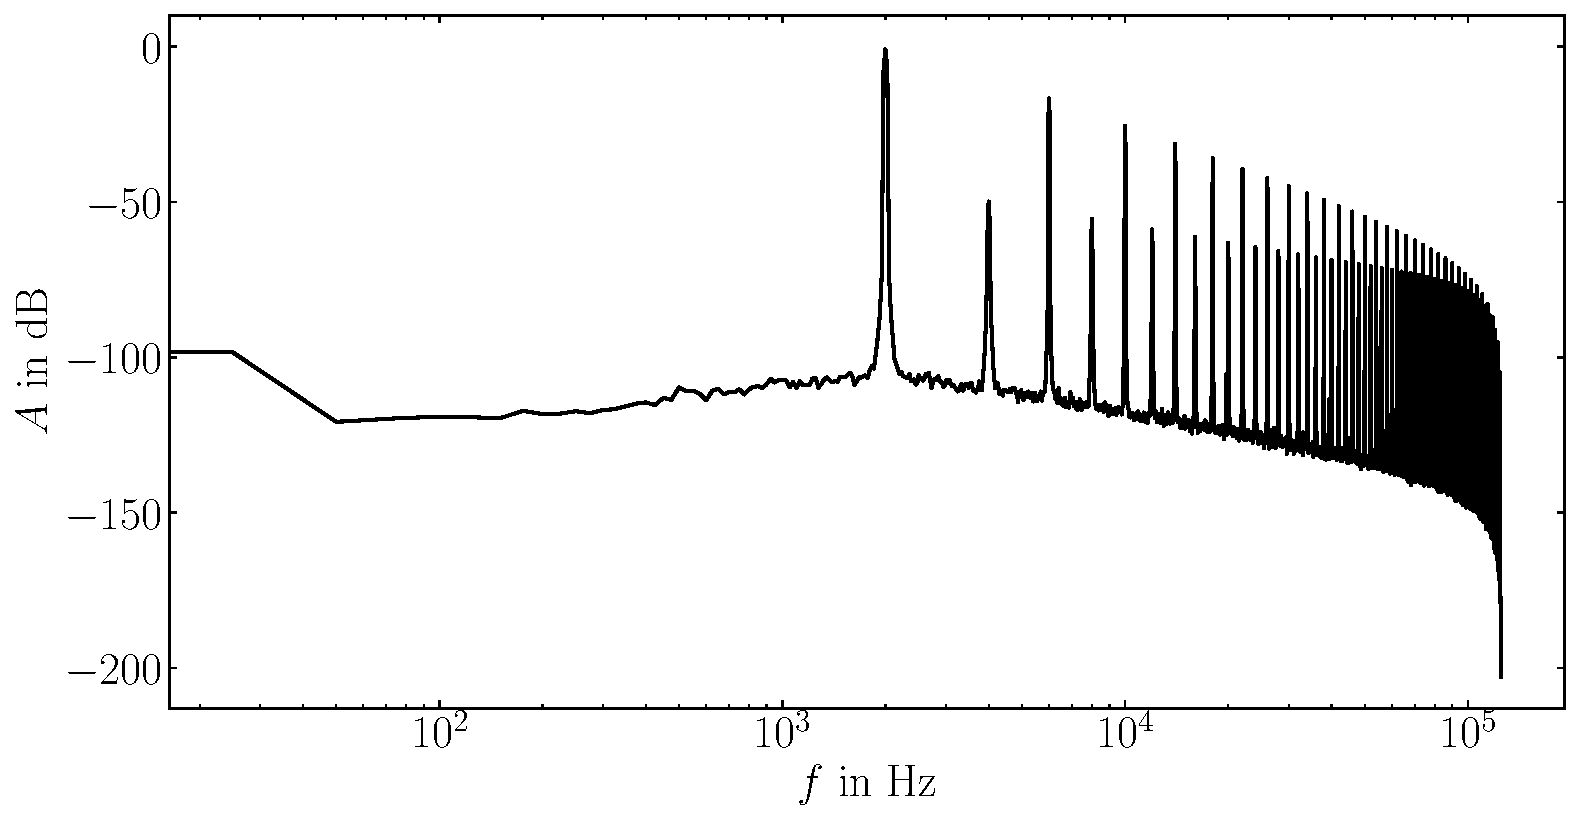
\includegraphics[width=\textwidth]{Paul/43eDF.pdf}
        \caption{digitale Filterung}
    \end{subfigure}
    \\
    \begin{subfigure}{0.9\textwidth}
        \centering
        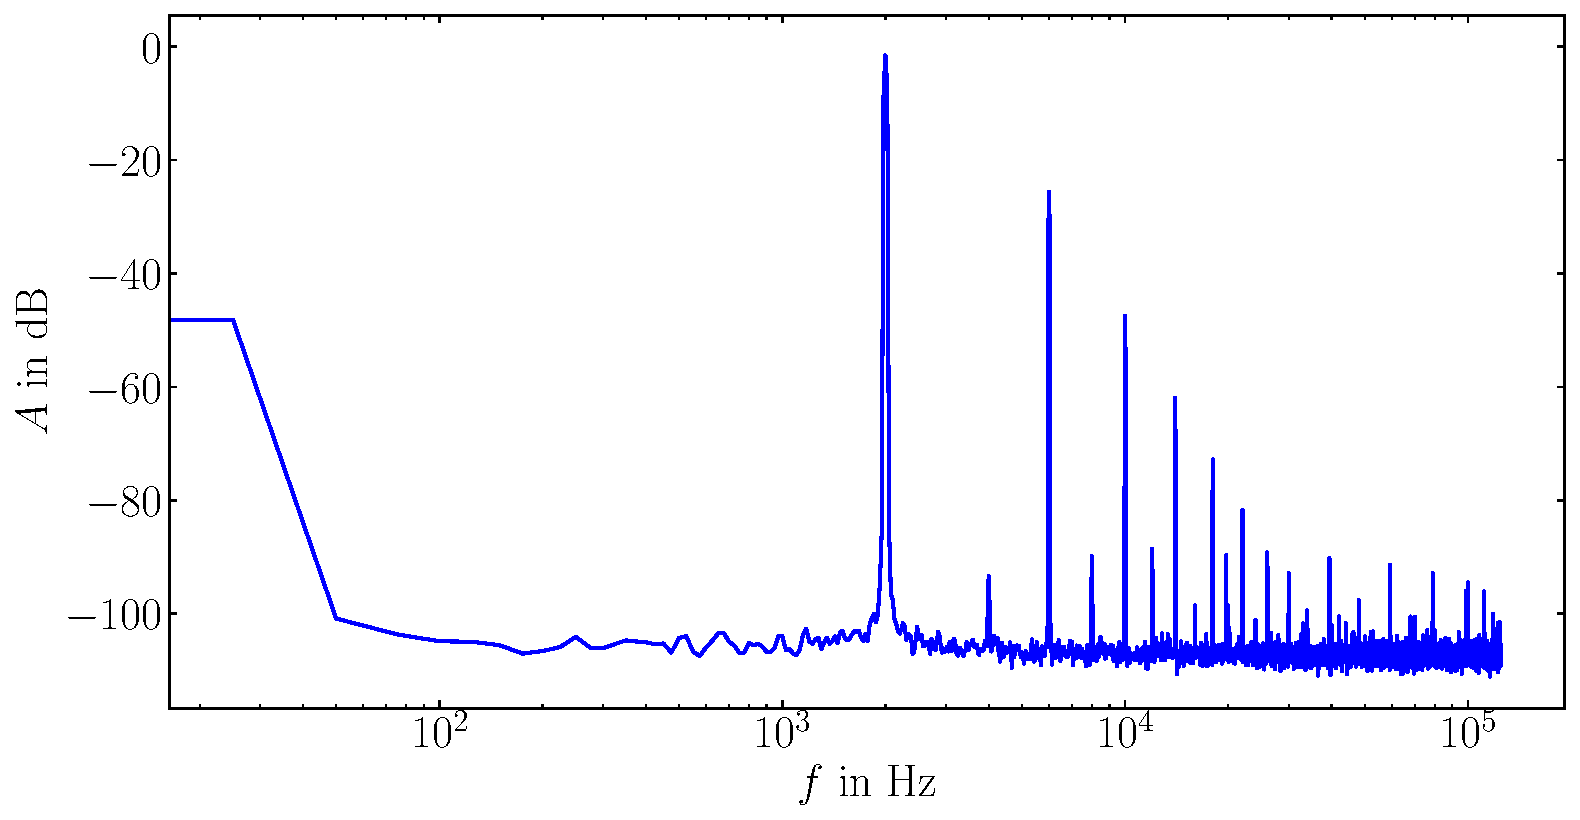
\includegraphics[width=\textwidth]{Paul/43eAF.pdf}
        \caption{analoge Filterung}
    \end{subfigure}
    \caption{Vergleich von analoger und digitaler Filterung}
    \label{fig:43e}
\end{figure}
\newpage
In Abbildung \ref{fig:43e} sind die Fourierspektren nach analoger und digitaler Filterung aufgetragen. Vergleicht man beides, so fällt auf, dass bei der digitalen Filterung auch der Hintergrund die Charakteristik des Bandpasses zeigt, wohingegen bei der analogen Filterung scheinbar nur die Nebenmaxima betroffen sind.\\
Eine mögliche Erklärung wäre, dass der Hintergrund nach dem analogen Filter einkoppelt oder das diese Eigenschaft eine Eigenschaft des analogen Filters ist.


\subsection{Vergleich Filterung und Mittelung}
Wenn man Filterung und Mittelung gegenüberstellt, so ist der größte Unterschied wohl das beim Filtern aktiv bestimmte Frequenzen unterdrückt werden, je nach Einstellung bzw. Dimensionierung des Filters. Dies kann dabei helfen, dass das Messsignal von Störungen wie dem 50 Hz Brummen bereinigt werden kann.\\
Mitteln hingegen ist besonders geeignet um die Messung von bspw. weißes Rauschen zu bereinigen da dies, gemittelt über die Zeit, null ergibt.